%!TEX TS-program = xelatex

\documentclass[xetex,mathserif,serif,t]{beamer}
% Если хотим соотношение сторон 16:9
% \documentclass[aspectratio=169,xetex,mathserif,serif,t]{beamer}

%%% Преамбула
\usetheme{MasterThesis} % Тема

%%% Работа с русским языком
\usepackage{fontspec,xunicode,xltxtra}

\defaultfontfeatures{Ligatures=TeX} % Для преобразования -- и ---
\setmainfont{PT Sans}
\setmonofont{PT Mono}

%%% Beamer по-русски
\newtheorem{rtheorem}{Теорема}
\newtheorem{rproof}{Доказательство}
\newtheorem{rexample}{Пример}

%%% Дополнительная работа с математикой
\usepackage{amsmath,amsfonts,amssymb,amsthm,mathtools} % AMS
\usepackage{icomma} % "Умная" запятая: $0,2$ --- число, $0, 2$ --- перечисление

%%% Свои команды
\DeclareMathOperator{\sgn}{\mathop{sgn}}

%%% Перенос знаков в формулах (по Львовскому)
\newcommand*{\hm}[1]{#1\nobreak\discretionary{}
{\hbox{$\mathsurround=0pt #1$}}{}}

%%% Работа с картинками
\usepackage{graphicx}    % Для вставки рисунков
\graphicspath{{../images/}} % Каталоги с картинками
\setlength\fboxsep{3pt}  % Отступ рамки \fbox{} от рисунка
\setlength\fboxrule{1pt} % Толщина линий рамки \fbox{}
\usepackage{wrapfig}     % Обтекание рисунков текстом

%%% Работа с таблицами
\usepackage{array,tabularx,tabulary,booktabs} % Дополнительная работа с таблицами
\usepackage{longtable}  % Длинные таблицы
\usepackage{multirow}   % Слияние строк в таблице

%%% Другие пакеты
\usepackage{lastpage} % Узнать, сколько всего страниц в документе
\usepackage{csquotes} % Еще инструменты для ссылок
\usepackage{multicol} % Несколько колонок
\usepackage{etoolbox} % Логические операторы

%%% Картинки
\usepackage{tikz,calc,ifthen,color}

\title{Исследование процессов обеспечения безопасности облачных сред}
\subtitle{Выпускная квалификационная работа магистра на тему:}
\author{Магистрант:\\
ст.гр.~ИВТ/м-31-з,~Умеров~А.Р. \\
\vspace{0.7\baselineskip}
Научный руководитель:\\
к.т.н.,~доцент,~Мащенко~Е.Н.}
\institute{Севастопольский государственный университет \\
Кафедра информационных технологий и компьютерных систем}
\date{2017~г.}

\begin{document}
%%% Содержимое слайдов

\frame[plain]{\titlepage} % Титульный слайд

%-------------------------------------------------------------------------------

\section{Цели и задачи исследования}

\begin{frame}
\frametitle{\insertsection}

\textbf{Цель:} повышение эффективности процессов обеспечения информационной безопасности облачных сред

\vspace{\baselineskip}

\textbf{Задачи:}
\begin{itemize}
    \item обзор составных частей облачной инфраструктуры
    \item анализ технологий используемых облачными провайдерами
    \item исследование специфики применений облачных вычислений в России
    \item исследование проблемы безопасности облачных вычислений
    \item исследование уязвимостей в облачной среде
\end{itemize}
\end{frame}

%-------------------------------------------------------------------------------

\section{Проблемы безопасности в облачной среде}

\begin{frame}
\frametitle{\insertsection}

\begin{itemize}
    \item утечка данных
    \item компрометация учетных записей и обход аутентификации
    \item взлом интерфейсов и API
    \item уязвимость используемых систем
    \item кража учетных записей
    \item инсайдеры-злоумышленники
    \item целевые кибератаки
    \item перманентная потеря данных
    \item недостаточная осведомленность
    \item злоупотребление облачными сервисами
    \item ...
\end{itemize}
\end{frame}

%-------------------------------------------------------------------------------

\section{Результаты системного и вариантного анализа}

\begin{frame}
\frametitle{\insertsection}

Системный анализ:
\begin{itemize}
    \item составление функций проектируемой облачной среды
    \item разбиение сложной системы на подсистемы
    \item детализация и декомпозиция подсистем
    \item учет изменяемости системы и случайностей в системе
\end{itemize}

\vspace{\baselineskip}

Вариантный анализ:
\begin{itemize}
    \item альтернативы: KVM, Hyper-V, VMware vSphere
    \item критерии: цена, масштабируемость, отказоустойчивость, интерфейсы управления
    \item предпочтение отдано альтернативе В (VMware vSphere)
\end{itemize}
\end{frame}

%-------------------------------------------------------------------------------

\section{Структурная схема облачной среды}

\begin{frame}
\frametitle{\insertsection}

\begin{figure}
    \center
    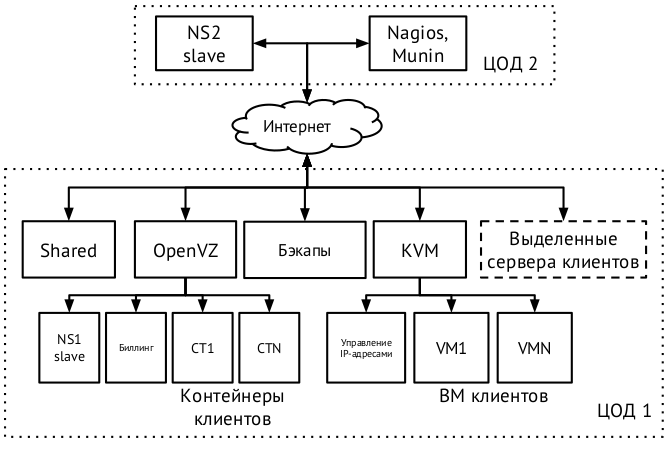
\includegraphics[width=\linewidth]{infrast-scheme}
\end{figure}
\end{frame}

%-------------------------------------------------------------------------------

\section{Архитектура информационной безопасности}

\begin{frame}
\frametitle{\insertsection}

\begin{figure}
    \center
    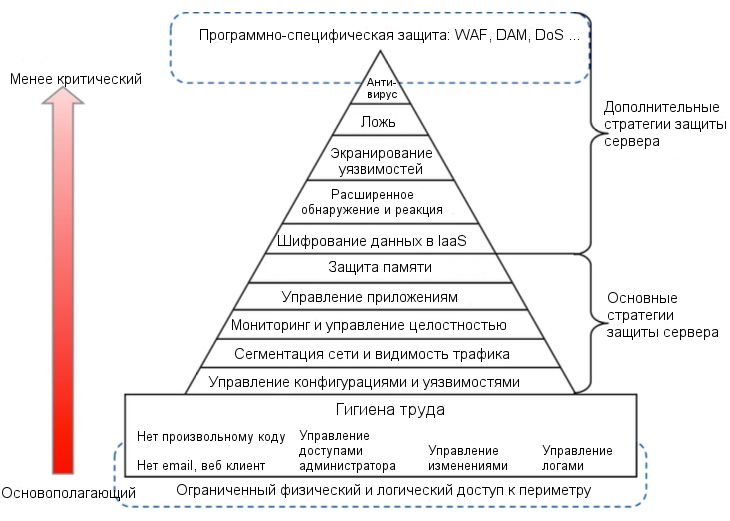
\includegraphics[width=\linewidth]{cwpp}
\end{figure}
\end{frame}

%-------------------------------------------------------------------------------

\section{Экспериментальные исследования}

\begin{frame}
\frametitle{\insertsection}
\framesubtitle{CVE-2016-5195}

{\small \texttt{\$ id \\
{\color{green} uid=1000(dcow)} gid=1000(dcow) groups=1000(dcow)
}}

\vspace{\baselineskip}

{\small \texttt{\$ g++ dcow.cpp -std=c++11 -pthread -lutil -o dcow \\
\$ ./dcow \\
Running ... \\
Received su prompt (Password: ) \\
Root password is: dirtyCowFun \\
Enjoy! :-)}}

\vspace{\baselineskip}

{\small \texttt{\$ su root \\
Password: dirtyCowFun \\
\# id \\
{\color{red} uid=0(root)} gid=0(root) groups=0(root)
}}
\end{frame}

%-------------------------------------------------------------------------------

\begin{frame}
\frametitle{\insertsection}
\framesubtitle{https://github.com/Amet13/vulncontrol}

{\scriptsize \texttt{\$ ./vulncontrol.py −d 2017−02−18 −m 5 -t \$TOKEN \$ID \\
CVE−2017−6074 9.3 http://www.cvedetails.com/cve/CVE−2017−6074/ \\
CVE−2017−6001 7.6 http://www.cvedetails.com/cve/CVE−2017−6001/ \\
CVE−2017−5986 7.1 http://www.cvedetails.com/cve/CVE−2017−5986/ \\
Telegram alert sent
}}

\begin{figure}
    \center
    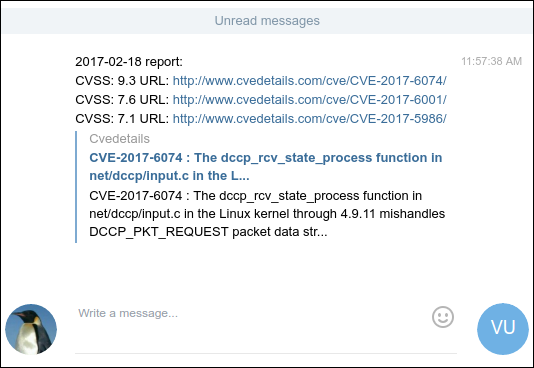
\includegraphics[width=0.65\linewidth]{tscreen}
\end{figure}
\end{frame}

%-------------------------------------------------------------------------------

\section{Результаты}

\begin{frame}
\frametitle{\insertsection}

\begin{itemize}
    \item обзор литературных источников и открытых стандартов
    \item анализ рынка облачных услуг
    \item определение угроз безопасности облачных вычислений и методов их решения
    \item системный анализ безопасности облачной среды
    \item вариантный анализ для выбора оптимальной альтернативы
    \item сбор данных по наиболее опасным уязвимостям в ПО
    \item практическая эксплуатация уязвимости CVE-2016-5195
    \item разработка системы сбора данных по уязвимостям
\end{itemize}
\end{frame}

%-------------------------------------------------------------------------------

\section{Выводы}

\begin{frame}
\frametitle{\insertsection}

\begin{itemize}
    \item не существует единого стандарта безопасности для провайдеров
    \item стоит уделить достаточно времени для анализа и выбора ПО
    \item российский облачный рынок стремительно развивается
    \item рост числа уязвимостей в ПО
\end{itemize}
\end{frame}

%-------------------------------------------------------------------------------

\frame[plain]{\titlepage}

%-------------------------------------------------------------------------------

\end{document}
